\documentclass[a4paper, 11pt]{article}
\usepackage{amsfonts, amsmath, amssymb, epsfig, subfigure, graphicx}
\usepackage{tikz}
\usetikzlibrary{calc,patterns}

\setlength{\textwidth}{6.5 in}
\setlength{\evensidemargin}{-.2500 in}
\setlength{\oddsidemargin}{-.2500 in}
\setlength{\textheight}{8.5 in}
\setlength{\topmargin}{-0.45 in}
\parindent=0pt
\parskip=10pt

%%%%% some useful shortcuts %%%%%%
\newcommand{\E}{\mathbb{E}}  % expected value
\newcommand{\R}{\mathbb{R}} % real numbers


\begin{document}
{\bf Information Theory, Master of Logic, UvA, Spring 2014} \\
Homework X \\
Student name here \\

\bigskip

1. Here is my solution to problem 1.... using loads of math like $I(X;Y) = \sum_{x,y} p(x,y) \log_2\left( \frac{p(x,y)}{p(x)p(y)}\right)$ or like
\[ I(X;Y) = \sum_{x,y} p(x,y) \log_2\left( \frac{p(x,y)}{p(x)p(y)}\right)\]
or even like this
\begin{align}
I(X;Y) &= \sum_{x,y} p(x,y) \log_2\left( \frac{p(x,y)}{p(x)p(y)}\right) \\
& = H(X) - H(X|Y) \\
& = H(Y) - H(Y|X)
\end{align}


\begin{tabular}[t]{p{.5\columnwidth}c}
Even entropy diagrams depicting $H(X)$, $H(Y)$ and $H(Z)$ are possible.
&
\raisebox{-14em}{
\begin{tikzpicture}[color=gray,fill=lightgray]
\footnotesize
\scope
\clip
      (2,0) circle (1.5)
      (-0.5,-3.5) rectangle (2.5,-0.5);
\clip 
      (0,0) circle (1.5)
      (-0.5,-3.5) rectangle (2.5,-0.5);
\fill 
      (1,-2) [pattern=dots, pattern color=lightgray] circle (1.5);
\endscope

\scope
\clip (.5,-1.5) rectangle (3.5,1.5)
      (0,0) circle (1.5);
\fill (2,0) [pattern=north east lines, pattern color=lightgray]  circle (1.5);
\endscope

\draw 
      (0,0) circle (1.5)  (0,1.5) node [text=black,above] {$H(X)$}
      (2,0) circle (1.5) (2,1.5)  node [text=black,above] {$H(Y)$}
      (1,-2) circle (1.5) (1,-3.5)  node [text=black,below] {$H(Z)$}
      (2.6,0)  node [text=black] {\parbox{2cm}{$H(Y|X)$}}
      (1,-2.2)  node [text=black] {$H(Z|XY)$}
      (0.3,-1.1)  node [text=black,rotate=30] {$I(X;Z|Y)$};
\end{tikzpicture}
}
\end{tabular}


\end{document}